% AUTO-GENERATED durch diagram_generator (L-c, echte-3D-Surface, z log-skaliert)
\begin{figure}[!htbp]
\centering
\resizebox{\textwidth}{!}{%
\begin{tikzpicture}
\begin{axis}[
    width=0.7800\textwidth,
    height=0.4000\textheight,
    scale only axis,
    title={3D-Rohdaten-Ansicht: Lookup-Latenz p50 (ns/op) (Suchalgorithmus x Workload)},
    xlabel={Workload},
    ylabel={Suchalgorithmus},
    grid=both,
    enlargelimits=0.05,
    view={45}{30},
    zmode=log,
    unbounded coords=jump,
    colorbar,
    colormap/viridis,
    zlabel={Lookup-Latenz p50 (ns/op)},
    xtick={0,1,...,0},
    ytick={0,1,...,0},
    xticklabels={ycsb\_c},
    x tick label style={rotate=45,anchor=east,font=\tiny},
    yticklabels={k\_ary},
    y tick label style={font=\tiny},
    mesh/cols=1,
    xmin=-0.5000, xmax=0.5000,
    ymin=-0.5000, ymax=0.5000,
    point meta min=750.0000, point meta max=7500.0000,
    zmin=750.0000, zmax=7500.0000,
]
% HONEST-EMPTY: z=nan = Zelle NICHT gemessen -> Loch im Mesh (unbounded coords=jump), KEIN
% Ersatzwert. Echte Messwerte stehen mit 4 Nachkommastellen -- auch die gemessene 0.0000.
\addplot3[surf] coordinates {
    (0,0,750.0000)

};
\end{axis}
\end{tikzpicture}
}%
\caption{3D-Rohdaten-Ansicht: Lookup-Latenz p50 (ns/op) (Suchalgorithmus x Workload)}
\end{figure}
